\section{Apéndices.}\label{apendice:tb_codigo}

\subsection{Salida del programa.}\label{apendice:salida}

Este es un ejemplo de salida obtenido al ejecutar el \anglicismo{script} del Apéndice~\ref{apendice:codigo:simulacion}. Concretamente esta salida se utilizó para obtener los valores que aparecen en la fila $e$ de la Tabla~\ref{tab:comparacion_porcentajes_1x}.

{\fontfamily{qcr}\selectfont

\small{

\vspace{5mm}
Random seed =  7

$\rho$ =  98.0 1 / mm3 

Volumen de la muestra:  250.0 mm3 

Diámetro droplet:  102.0 micron 

Flujo fase dispersa:  3.0 mm3 / min 

Número de simulaciones:  4 

Desviación estándar relativo al tamaño de la droplet expresado como tanto 

por 1: 0.16 

\vspace{5mm}

Volumen droplet:  0.0005556472094551194 mm3 

Duración experimento:  83.33333333333333 min 

Tasa de formación:  89.98515451743413 1 / s 

\vspace{5mm}

Simulación | Tiempo transcurrido | elementos | repeticiones | n-droplets

1 .  0:00:06.390786 [0 1 2 3] [426120  23182    656     11] 449969

2 .  0:00:12.518754 [0 1 2 3] [426130  23137    673      7] 449947

3 .  0:00:18.676374 [0 1 2 3] [425938  23213    631     10] 449792

4 .  0:00:24.851280 [0 1 2 3] [425959  23181    645     11] 449796

\vspace{5mm}

A partir de las simulaciones anteriores:

Células/droplet | Promedio de n-droplets $\pm$ desviación estándar

  0   426036 $\pm$ 88
  
  1   23178 $\pm$ 27
  
  2   651 $\pm$ 15
  
  3   9 $\pm$ 1
  
\vspace{5mm}

El número de encapsulados múltiples representa el  2.8097462060336738 \% de

los encapsulados únicos.

\vspace{5mm}

El número de encapsulados múltiples representa el 2.732957049035859 \% de 

los encapsulados totales. Nuestro objetivo es que se encuentre en el 5\%.

\vspace{5mm}

Porcentaje que representa cada conjunto de droplets con distinto número 

de encapsulados respecto del total de la muestra:

 [94.71777205666568, 5.1530582753070275, 0.1447878593851435,
 
 0.002167649334364912]
 
}% del small
 
\vspace{5mm}
}

\vspace{-7mm}

\begin{figure}[H]
    \begin{center}
         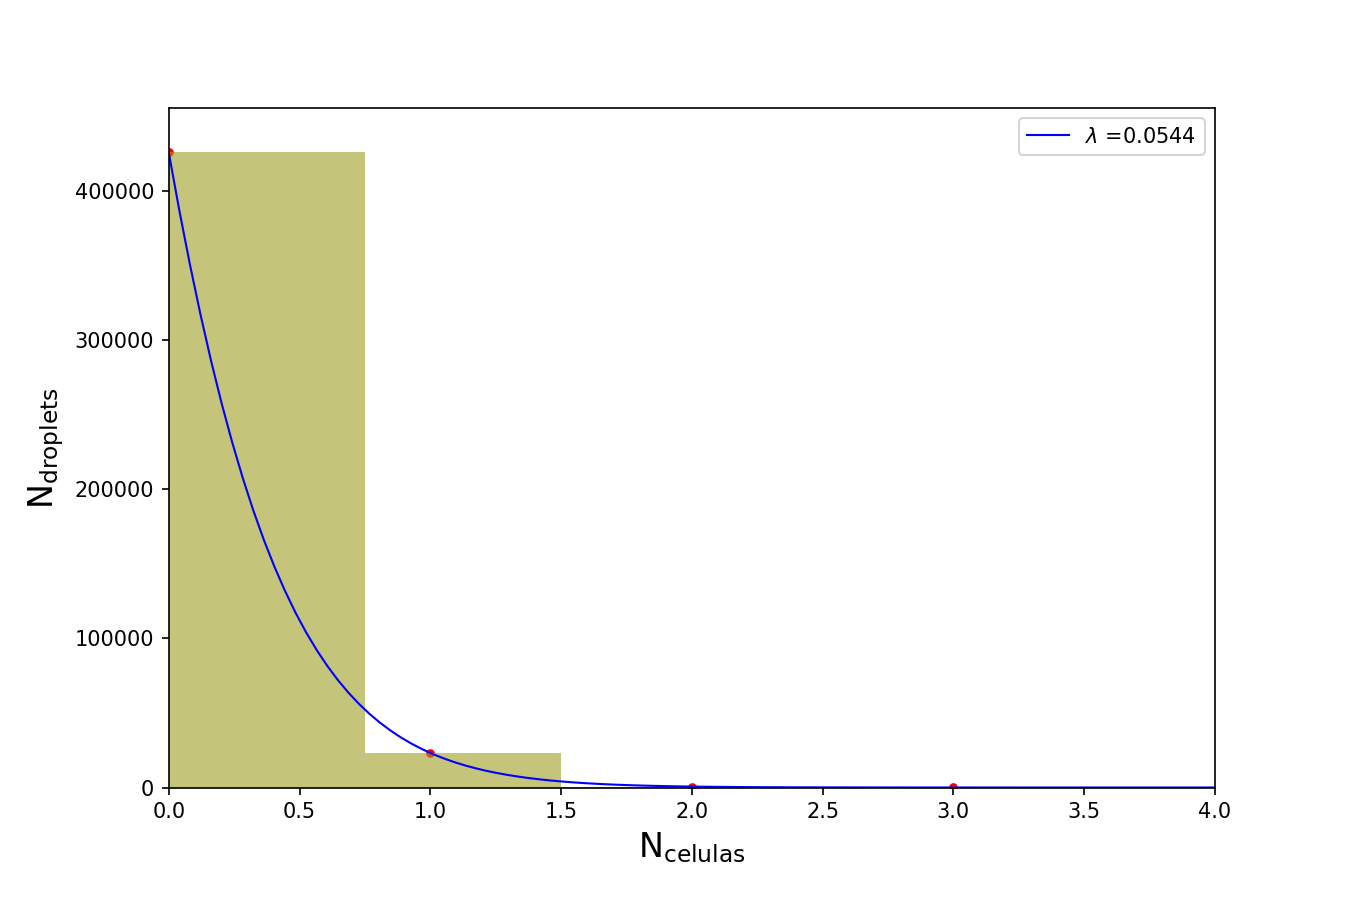
\includegraphics[angle=0,width=0.9\textwidth]{4_resultados/histograma_1x.png}
    \end{center}
\end{figure}



% Los programas que se presentan en esta sección contienen todo lo necesario para realizar todos los cálculos y gráficas a los que se ha hecho referencia en las secciones anteriores; están escritos en lenguaje de programación \texttt{Python 3.6.0} y se requiere tener instaladas las librerías \texttt{scipy 0.18}, \texttt{matplotlib 2.0.0}, \texttt{numpy 1.11.3} y \texttt{astropy 1.3}.

% Las gráficas sirven para comprobar de forma gráfica y rápida que el comportamiento del programa es el razonable y la distribución de medias se ajusta a los valores teóricos que esperamos a partir de lo que ya sabemos (un buen ajuste a la distribución de poisson)

% El ajuste a la distribución de poisson es muy bueno cuando las concentraciones de células son bajas, independientemente del algoritmo que utilicemos (me refiero a encapsuladosss o encapsuladossw). Esto refuerza la idea de que los dos algoritmos, aunque aparecen ciertas diferencias funcionan correctamente (que los recuentos se ajusten a la distribución de poisson verifica de alguna manera que ambos programas hacen correctamente los recuentos).

% \begin{minted}{python}
%     >>> help("nombre_modulo.nombre_funcion")
% \end{minted}

% \vspace{-4mm}

% o

% \vspace{-4mm}

% \begin{minted}{python}
%     >>> print(nombre_funcion.__doc__)
% \end{minted}

% \vspace{-2mm}

% Para facilitar la comprensión del código en la medida de lo posible, también se han realizado dos esquemas sobre la estructura de los ejecutables \texttt{main\_halos.py} (\ref{apendice:esquema_main_halos}) y \texttt{main\_matching.py} (\ref{apendice:esquema_main_matching}) que son quizás, los que tienen mayor complejidad.



\subsection{\anglicismo{Script} \texttt{simulacion.py}}\label{apendice:codigo:simulacion}

\inputminted{python}{apendices/codigo/densidad_celulas_13_sigma_definitivo}\label{apendice:codigo:script}



\subsection{Código para la placa de Arduino.}\label{apendice:codigo:arduino}

\inputminted{python}{apendices/codigo/tfm_definitivo.cpp}
